\documentclass[
,hyperref={pdfpagelabels=false}
,xcolor=dvipsnames
]{beamer}
% Die Hyperref Option hyperref={pdfpagelabels=false} verhindert die Warnung:
% Package hyperref Warning: Option `pdfpagelabels' is turned off
% (hyperref)                because \thepage is undefined.
% Hyperref stopped early

\usepackage{agstyle}
\usepackage{currycode}

\newcommand{\ergo}{$\Rightarrow$}
% \newcommand{\todo}[1]{{\bfseries TODO:} #1}

\newcommand{\pro}{\makebox[1ex]{\color{Green}\bfseries +}}
\newcommand{\con}{\makebox[1ex]{\color{Red}  \bfseries \textendash}}

%%%%%%%%%%%%%%%%%%%%%%%%%%%%%%%%%%%%%%%%%%%%%%%%%%%%%%%%%%%%%%%%%%%%%%%%%%%%%%%%

\title{Tracing Failure in KiCS2}
\date{December 05, 2012}
\author{Björn Peemöller}
\institute{Kiel University}

\begin{document}

\begin{frame}[fragile]%-------------------------------------------------------
\titlepage
\end{frame}


\begin{frame}[fragile]%-------------------------------------------------------
\frametitle{Failures in FLP}

\begin{itemize}

\item Functional Programming
\begin{itemize}
\item Failure corresponds to illegal arguments/error
\item Stops execution
\end{itemize}

\item Logic Programming
\begin{itemize}
\item Common programming pattern to mark invalid computations
\item Handled by top-level search
\end{itemize}

\item Functional-Logic Programming
\begin{itemize}
\item Failure in functional-logic part is handled by (top-level) search
\item Failure in IO part is reported
\end{itemize}

\end{itemize}
\end{frame}


\begin{frame}[fragile]%-------------------------------------------------------
\frametitle{Unexpected Failures in Curry Programs}

\blocktitle{In deterministic programs}
\begin{example}[The KiCS2 Curry compiler]
\begin{program}
> bin/kics2c -i lib/ -i meta/ Prelude.curry
kics2c: FailException "{}IO action failed"
\end{program}
\end{example}

\pause
\medskip

\blocktitle{In non-deterministic programs}
\begin{example}[Solving the N queens problem]
\begin{program}
> ./nqueens 8
No more solutions.
\end{program}
\end{example}

\pause
\medskip

\begin{center}
\ergo{} Demand for better failure reporting
\end{center}
\end{frame}


\begin{frame}[fragile]%-------------------------------------------------------
\frametitle{Sources for Failure}

\begin{curry}[Incomplete pattern matching]
head :: [a] -> a
head (x : _) = x
\end{curry}

\begin{curry}[Illegal parameters]
div x 0 = failure "{}Division by Zero"
\end{curry}

\begin{curry}[Failing unification]
0  =:= 1      --- clash
xs =:= (x:xs) --- occur check
\end{curry}

\begin{curry}[Explicit failure]
f [] = failed
\end{curry}
\end{frame}


\begin{frame}[fragile]%-------------------------------------------------------
\frametitle{Runtime Representation of Failure}

Failures are explicitly represented in data structures

\begin{curry}
data Bool = True | False

ensureTrue True = True
\end{curry}

\begin{haskell}
data Bool = True | False | Choice ID Bool Bool | \alert{Fail}

ensureTrue True             = True
ensureTrue (Choice i x1 x2) = Choice i (ensureTrue x1)
                                       (ensureTrue x2)
\alert{ensureTrue _                = Fail}
\end{haskell}
\end{frame}

\begin{frame}[fragile]%-------------------------------------------------------
\frametitle{Recording the Failure Cause}

\begin{itemize}
\item \verb!Fail! constructors are augmented with additional information
\item Incomplete pattern matching reports unmatched pattern
\item Anagously for invalid parameters, unification, \verb!failed!
\end{itemize}

\pause

\begin{haskell}
data FailInfo = FailInfo \{ failCause :: String \}
\end{haskell}

\begin{haskell}
data Bool = True | False | Choice ID Bool Bool | Fail \alert{FailInfo}

ensureTrue True             = True
ensureTrue (Choice i x1 x2) = Choice i (ensureTrue x1)
                                       (ensureTrue x2)
ensureTrue x                = Fail \alert{(consFail "{}ensureTrue" (showCons x))}
\end{haskell}
\end{frame}

\begin{frame}[fragile]%-------------------------------------------------------
\frametitle{Tracing the Call Stack}

\begin{itemize}
\item A call stack represents the expressions whose evalution led to failure
\item The call stack is extended at pattern matching
\end{itemize}

\pause

\begin{haskell}
type Call     = (String, [String])
data FailInfo = FailInfo \{ failCause :: String\alert{, failTrace ::  [Call]} \}
\end{haskell}

\begin{haskell}
ensureTrue True             = True
ensureTrue (Choice i x1 x2) = Choice i (ensureTrue x1)
                                       (ensureTrue x2)
\alert{ensureTrue (Fail info)      = Fail (addTrace "{}ensureTrue" info)}
ensureTrue x                = Fail (consFail "{}ensureTrue" (showCons x))
\end{haskell}

\end{frame}

\begin{frame}[fragile]%-------------------------------------------------------
\frametitle{Intermediate Result}

The mentioned scheme

\begin{itemize}
\item[\pro] reports the cause of failure
\item[\pro] traces failures in argument positions
\item[\pro] does not introduce overhead for non-failing programs
\item[\con] no tracing information for functions that
\begin{itemize}
\item project a failing argument
\item have a failing right-hand-side
\end{itemize}
\end{itemize}

\pause

\vspace{-.5cm}

\begin{columns}[t]
\column{.45\textwidth}
\begin{example}[Projecting Failure]
Given the function
\begin{program}
f x = [x]
\end{program}
\verb!f! is not traced in \verb!f failed!
\end{example}

\pause

\column{.45\textwidth}
\begin{example}[Failing RHS]
Given the function
\begin{program}
f 0 = head []
\end{program}
\verb!f! is not traced in \verb!f 0!
\end{example}
\end{columns}
\end{frame}


\begin{frame}[fragile]%-------------------------------------------------------
\frametitle{Adding Failure Checking}

Every function is augmented with a failure check at top-level

\begin{itemize}
\item[\pro] Function with failing RHS is traced
\item[\pro] Strictness property of function is preserved
\item[\con] Considerable runtime overhead \ergo{} only in debug mode
\end{itemize}

\pause

\begin{curry}
ensureTrue True = True
\end{curry}

\begin{haskell}
ensureTrue x = \alert{failCheck "{}ensureTrue" [show x]} (case x of
  True           -> True
  Choice i x1 x2 -> Choice i (ensureTrue x1) (ensureTrue x2)
  Fail info      -> Fail info
  _              -> consFail "{}ensureTrue" (showCons x))
\end{haskell}
\end{frame}

\begin{frame}[fragile]%-------------------------------------------------------
\frametitle{Evaluation of the Call Stack}

\blocktitle{Directly printing the call stack}

\begin{itemize}
\item may flood the output
\item may not terminate due to
\begin{itemize}
 \item non-terminating argument evaluation
 \item infinite data structures
\end{itemize}
\end{itemize}

\pause

\blocktitle{Therefore, in case of failure}

\begin{itemize}
\item the failure cause gets reported
  \item the call stack shows the function names
  \item the arguments are evaluated on user demand
\end{itemize}

\end{frame}

\begin{frame}%----------------------------------------------------------------
\frametitle{Benchmark: Performance Impact of Tracing}

\begin{center}
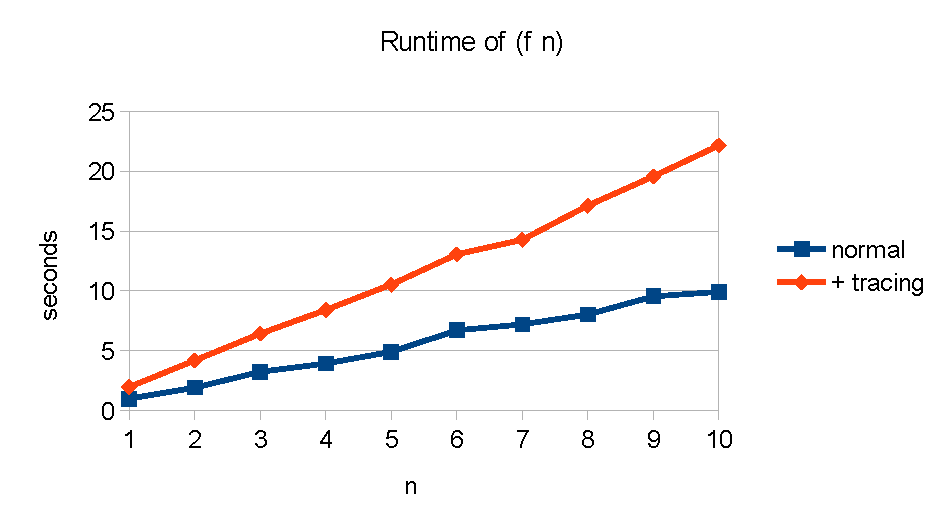
\includegraphics[width=11cm]{benchmark}
\end{center}

\vspace{-.5cm}

\begin{curry}[Test program]
f n = last [1 .. 1000000 * n]
\end{curry}

\bigskip

\end{frame}


\begin{frame}[fragile]%-------------------------------------------------------
\frametitle{Conclusion}

\blocktitle{Summary}
\begin{itemize}
\item Failure reporting gives valuable information to the user
\item Interactive evaluation of trace information
\item Projection of failure currently not traced
\end{itemize}

\blocktitle{Possible Improvements}
\begin{itemize}
\item Use Haskell debugging mechanisms (Hood, Hat)
\item Integrate existing debugging tools for Curry (CooSy)
\end{itemize}

\end{frame}

\end{document}
